\chapter{Methodology}
\label{sec:methodology}

As the endeavor of this thesis was the merger and enhancement of various aspects of the LORNA project, the complexity lied rather in the understanding of the existing work and the interfaces thereof as opposed to the challenging methodology pursued in the novel contributions. Therefore, the implementation aspect of this work carries more weight than the theoretical decision-making associated with it.

The autonomy framework\citep{Autonomy} allows us to fly independent missions at cruise altitude of 100+ m. The structure from motion approach captures 3D information during traversal as its adaptive baseline allows it to perceive high quality depth information also at such high altitudes. This information can be used by LSD in order to detect landing sites during mission. 

At low altitudes SFM works as well but surrounded with obstacles, the need for lateral motion poses significant risk. This is because a local state estimator is by nature prone to accumulate an estimation error and the same holds for the structure from motion approach. Our terrain knowledge can thus become void. 

To overcome this issue, a range sensor can be used. As LiDAR might come to mind. However, a LiDAR sensor produces rather sparse point clouds unless a newer sensor like for instance Ouster's OS1-128 sensor is used. In that case, there remains the weight issue with the sensor's 495g. As the drone is going to fly on Mar's very thin atmosphere, this isn't feasible. 

Staying with the project's theme of visual sensors, a stereo camera poses a solution as it offers in-place triangulation with a very low weight ($\tilde 10g$). Therefore, in this thesis I present a stereo camera range node implementation to remedy the shortcomings at low altitudes.

% This is because the drone does not retain any hazard information past the knowledge of detected landing sites and terrain knowledge from either HiRISE, Ingenuity or the rover which is implicitly used for the mission creation. Therefore, it could be said that the drone flies blindly with respect to obstacles. 

\section{Stereo Camera}\label{sec:stereo_methodology}

The implementation of the stereo camera sensor itself is very straightforward as simply duplicating an existing camera, offsetting it an adequate distance to resemble the real model, and setting the parameters to equal the hardware, results in the desired outcome.

The simulated camera sensors used for this had the following properties:

\begin{itemize}
    \item Image width: 640 pixels
    \item Image height: 480 pixels
    \item fx: 275.42px
    \item fy: 276.27px
    \item cx: 342.22
    \item cy: 234.66
\end{itemize}

The input to the stereo camera depth node are the two camera images and the drone's base link pose. Processing this information is different from for the existing SFM algorithm. Therefore, a new depth generation node was put in place. 

As mentioned in \cref{sec:rel_stereo}, state-of-the-art deep learning based stereo depth methods have considerably higher computational overhead. Due to the embedded CPU's computation limitations, this restricts us to using classical algorithms such as OpenCV's implementations of Heiko Hirschmüller's approach (\citep{Stereo}).

The initial goal of the stereo camera implementation of this work was to show proof of concept for this approach of depth detection without lateral motion. Due to personal experience with the OpenCV library, the initial choice of stereo depth method was OpenCV's StereoSGBM algorithm. This algorithm is introduced in \cref{subsec:disparity_creation}.

JPL has its own visual library called JPLV containing a stereo matching method which might be a more adequate choice for the future. This is because throughout various projects at JPL, issues with the StereoSGBM algorithm occurred. \textbf{\@ Roland: Which?}
Also, JPLV contains implementations for the often used CAHVORE camera model which OpenCV natively does not support. However, for the time of this work, especially using camera images without distortion, there was no specific reason to switch away from the working StereoSGBM implementation, therefore, the continuation thereof was pursued.

Furthermore, OpenCV's StereoBM variation was considered which is in general faster but less accurate than StereoSGBM. An analysis thereof is shown in \cref{subsec:bmvssgbm}.


\subsection{Stereo Camera Advantages}

The specific advantage of a stereo camera implementation when compared to SFM can be summarized in the following points:

\begin{itemize}
    \item No necessity of lateral motion
    \item Hardware depth perception
    \item DEM conversion
    \item Efficiency
\end{itemize}

\subsubsection{Lateral Motion}

As already mentioned above the need for lateral motion in itself is an undesirable necessity for a rotorcraft in unknown terrain. 

In this setup the structure from motion approach is based on a key frame buffer which needs to be filled with image-pose pairs at different horizontal positions in order to start acquiring depth information. The current setting in the implementation \citet{SFM} uses 6 key frames. Therefore, for a single point cloud it is necessary to move laterally 6 times in order to start perceiving depth. Following the depth error formula from a stereo disparity image (\ref{eq:SFM_depth_error}) and assuming an altitude of 2.5 m above ground with a focal length of 256 pixels and a disparity error of 0.5 pixels, the necessary baseline in order to keep the depth error below a critical 5 cm is:

\subsubsection{Software vs Hardware Depth Perception}

Structure from Motion, being a software node that relies on camera poses supplied by a state estimator, is by design subject to inaccuracies. A depth node based on a stereo camera on the other hand works with a fixed rigid baseline between the camera views. Thus, for low altitude flights that bear the danger of collision, a more robust hardware approach is preferred.

\subsubsection{DEM Conversion}

As described in \cref{subsubsec:setup:aggregation} the multi-resolution DEM used for depth aggregation in LSD is based on Optimal Mixture of Gaussian cells and thus converges over time. 

According to \cref{subsubsec:setup:haz_seg} the landing sites chosen are likely on terrain with low uncertainty. Because of this landing sites are more likely to be detected and have in general a better quality when the terrain perceived has been viewed.

When a landing site has been selected we need to make sure that the landing site is actually correctly detected and of good quality. For this we would like to (re-)detect landing sites on rather converged terrain. Structure from Motion needs constant lateral motion for this. A stereo camera depth node simply hovers in place for any given amount of time.

\subsubsection{Efficiency}

All in all the stereo camera setup allows us to perceive a landing site at course altitude and after having traversed horizontally to that location, we can simply descend to a stereo camera friendly altitude for the verification. Compared to repeated lateral coverage of the area in question this is a huge increase in efficiency.

Looking in depth at the stereo alternative of depth generation, we can first analyze the theoretical threshold of this system.

\section{Ground Truth Depth}

For evaluation purposes as well as proof of concept aspirations, a ground truth is required. 

Additionally, GT was important, because at the time of this work the structure from motion node showed frequent signs of unreliability. See \cref{subsec:sfm_insufficiencies} for the evaluation thereof.

\subsection{Ground Truth Implementation}
The simulation already supplied the ground truth pose of the drone's base link through the ROS bridges. When applying the static camera transform to it, this yielded the ground truth camera pose. Using Gazebo's depth camera sensor\footnote[1]{As there was a bug in Gazebo's source code, the depth camera couldn't be used out of the box. More on this in \cref{chapter:appendix:gz_depth_camera}.}, a ground truth point cloud could be created.

The depth camera creates the image using traced rays which fill a pixel with the center most range value that a ray detected.

As expected, the ground truth point clouds yielded very clean and easily interpretable LSD DEMs:

\begin{figure}[h]
\centering
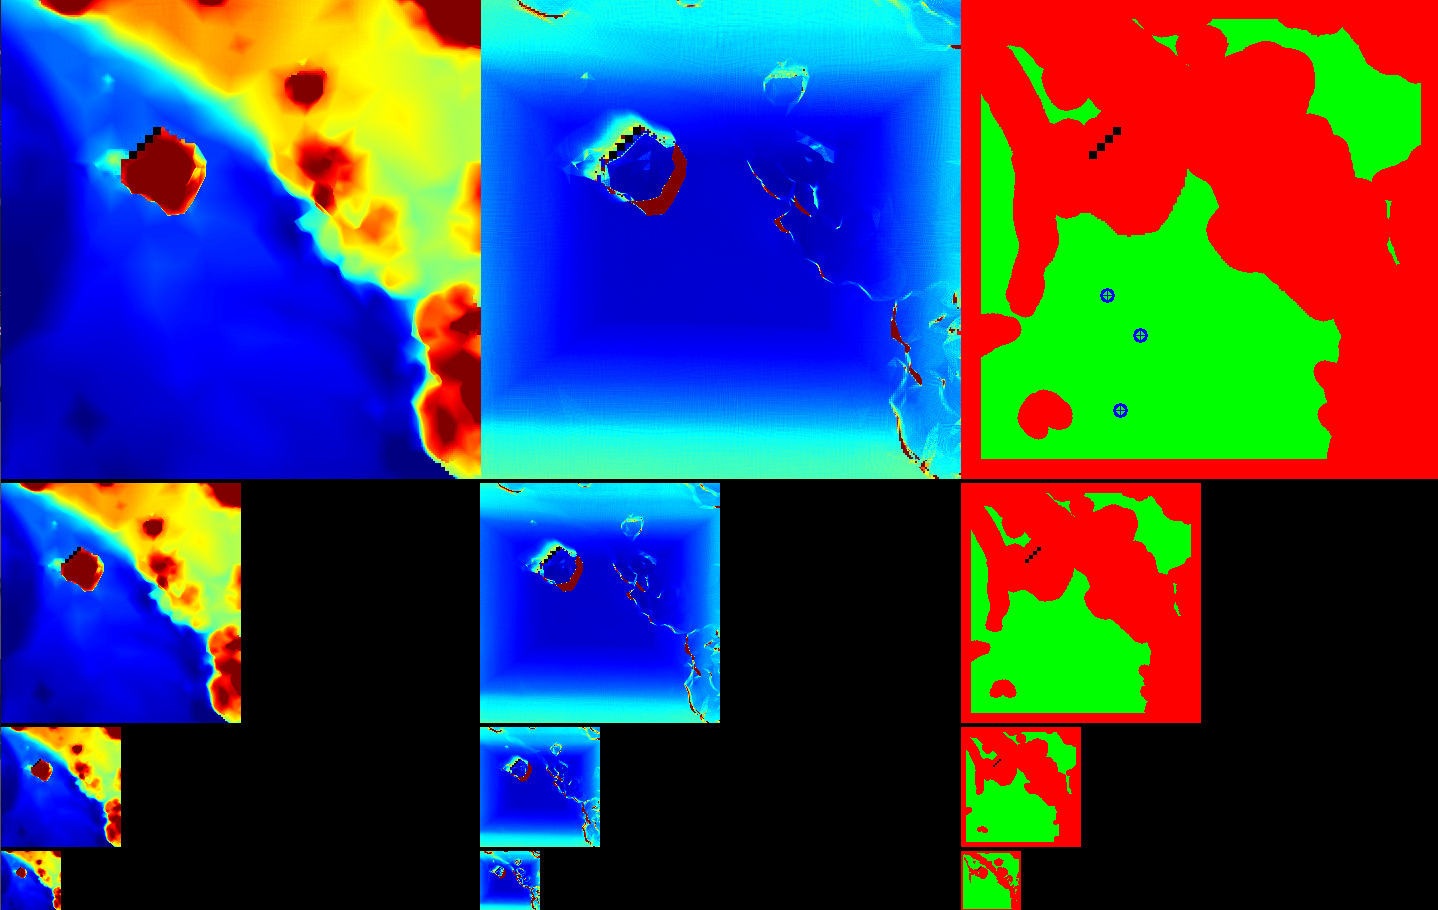
\includegraphics[scale=0.25]{images/methodology/lsd_debug_image.png}
\caption{LSD debug image using a GT point cloud}
\label{fig:gt_lsd_debug}
\end{figure}

\begin{figure}[h]
\centering
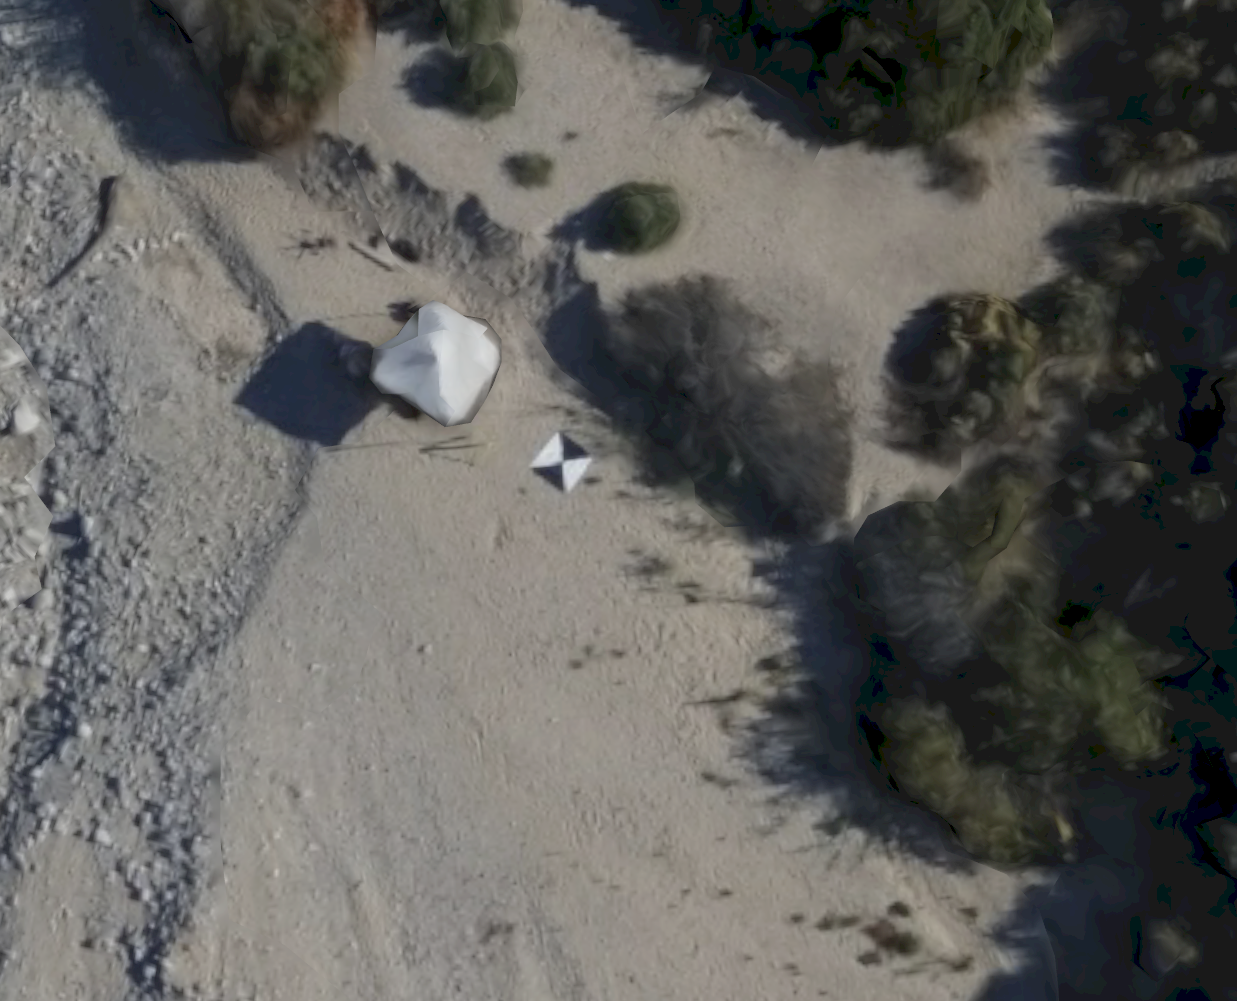
\includegraphics[scale=0.25]{images/methodology/lsd_debug_reference.png}
\caption{LSD debug image simulation terrain reference}
\label{fig:gt_lsd_debug_reference}
\end{figure}
\clearpage %HERE

\subsection{Comparability to SFM}

This is sufficient for a qualitative analysis of the stereo depth node. However, to use the ground truth as an alternative for SFM, one has to make sure that the GT quality is not too good. For instance, SFM, like the stereo camera depth, has a depth error associated with its point cloud creation. At high altitudes this can lead to the neglect of small (but for the drone threatening) rocks. So, in order to test the autonomous landing pipeline with ground truth, I had to make sure that small rocks of about 10 cm diameter were not seen by the GT at a cruise altitude of 100 m.

For this, the following test was designed.

On the Arroyo map, three cylinders of different sizes were placed. On each cylinder a small rock of 10 cm diameter was placed. The drone was then flown over the test setup up 100 m altitude to detect the scene once with SFM and once using the GT depth. The goal was to find out, whether the ground truth depth quality would have to be artificially decreased, using Gaussian or median filtering for instance, in order to make it more comparable to SFM.

\begin{figure}[ht]
\centering
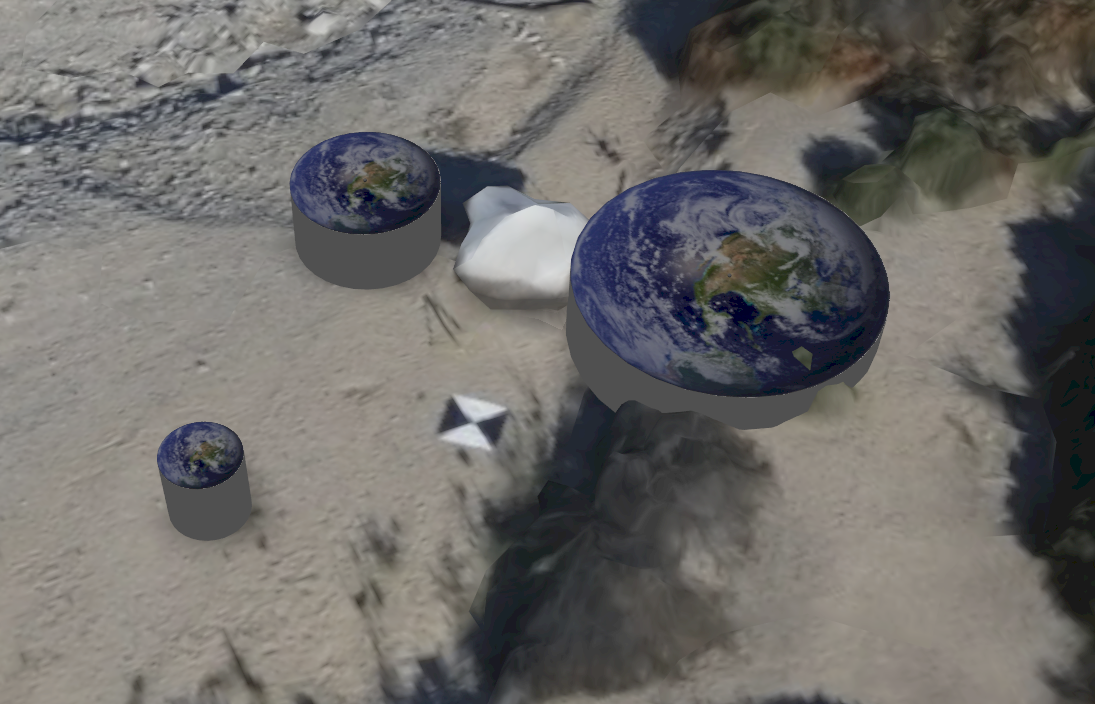
\includegraphics[scale=0.3]{images/methodology/test_setup1.png}
\caption{GT test setup1: Three cylinders of different sizes (4, 2 and 1 m diameter) were placed on the map}
\label{fig:gt_test_setup1}
\end{figure}

\begin{figure}[ht]
\centering
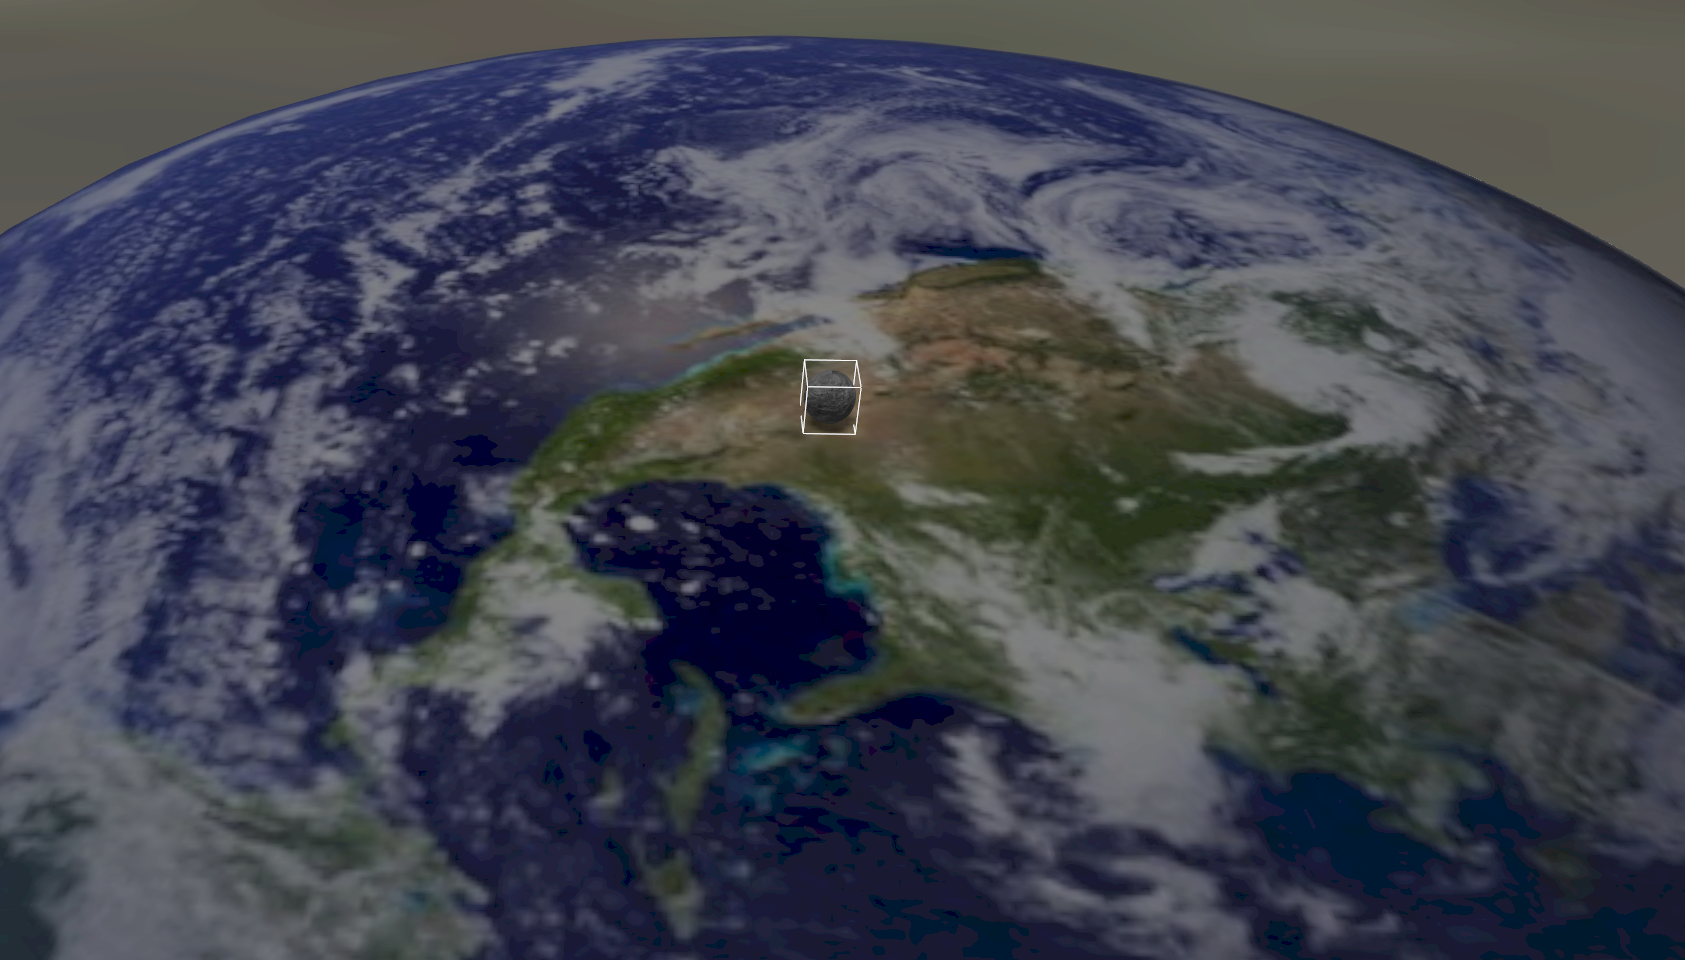
\includegraphics[scale=0.18]{images/methodology/test_setup2.png}
\caption{In the middle of each cylinder a rock of 10 cm diameter was placed}
\label{fig:gt_test_setup2}
\end{figure}

\begin{figure}[ht]
\centering
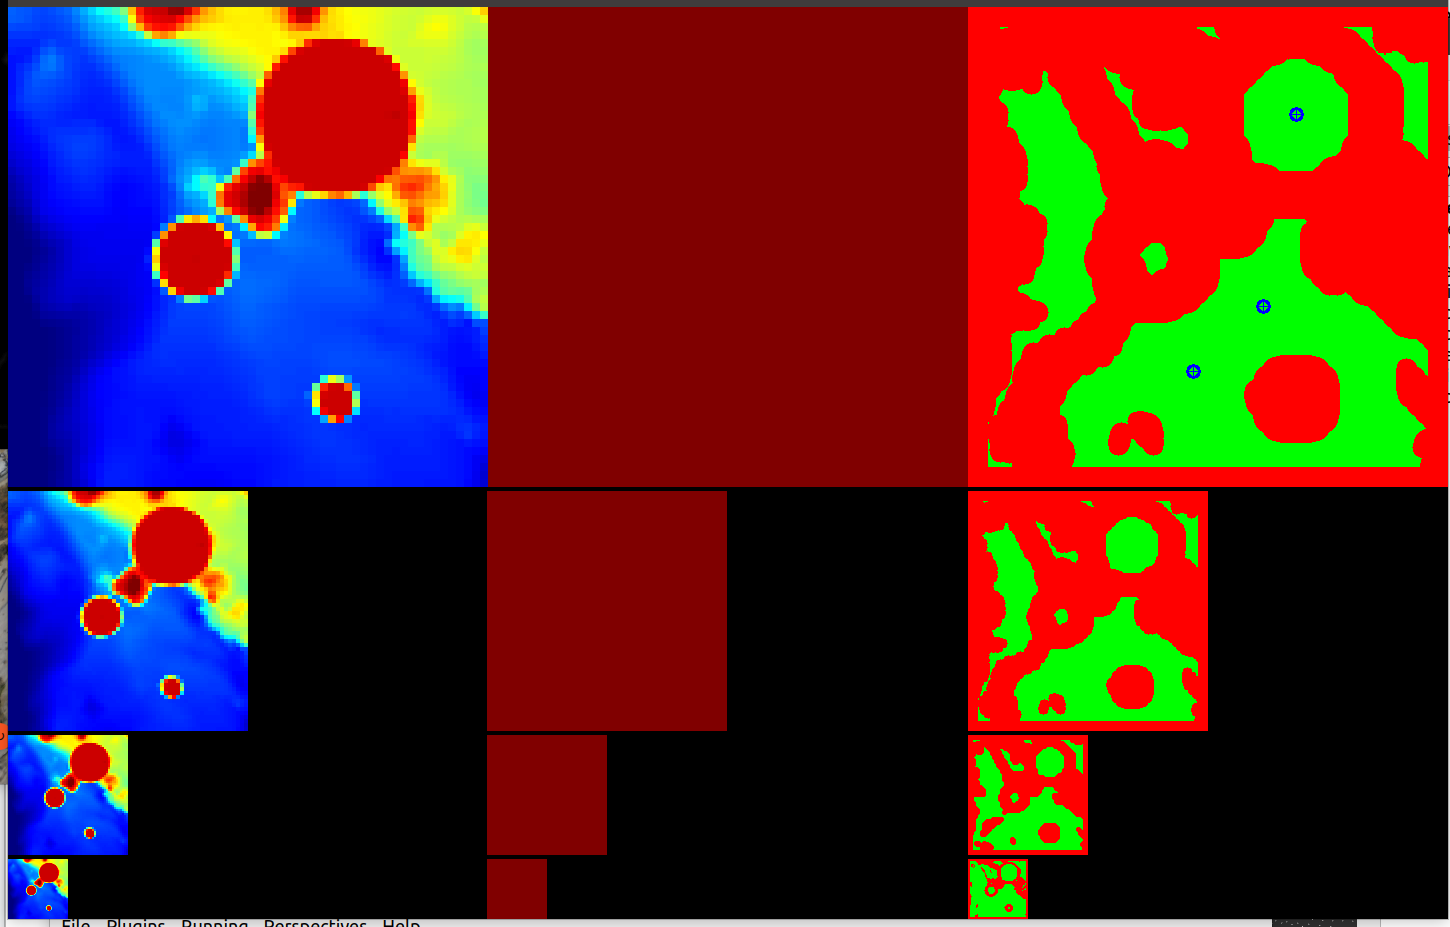
\includegraphics[scale=0.22]{images/methodology/GT.png}
\caption{Ground truth result of the GT test}
\label{fig:gt_test_gt} 
\end{figure}

\begin{figure}[ht]
\centering
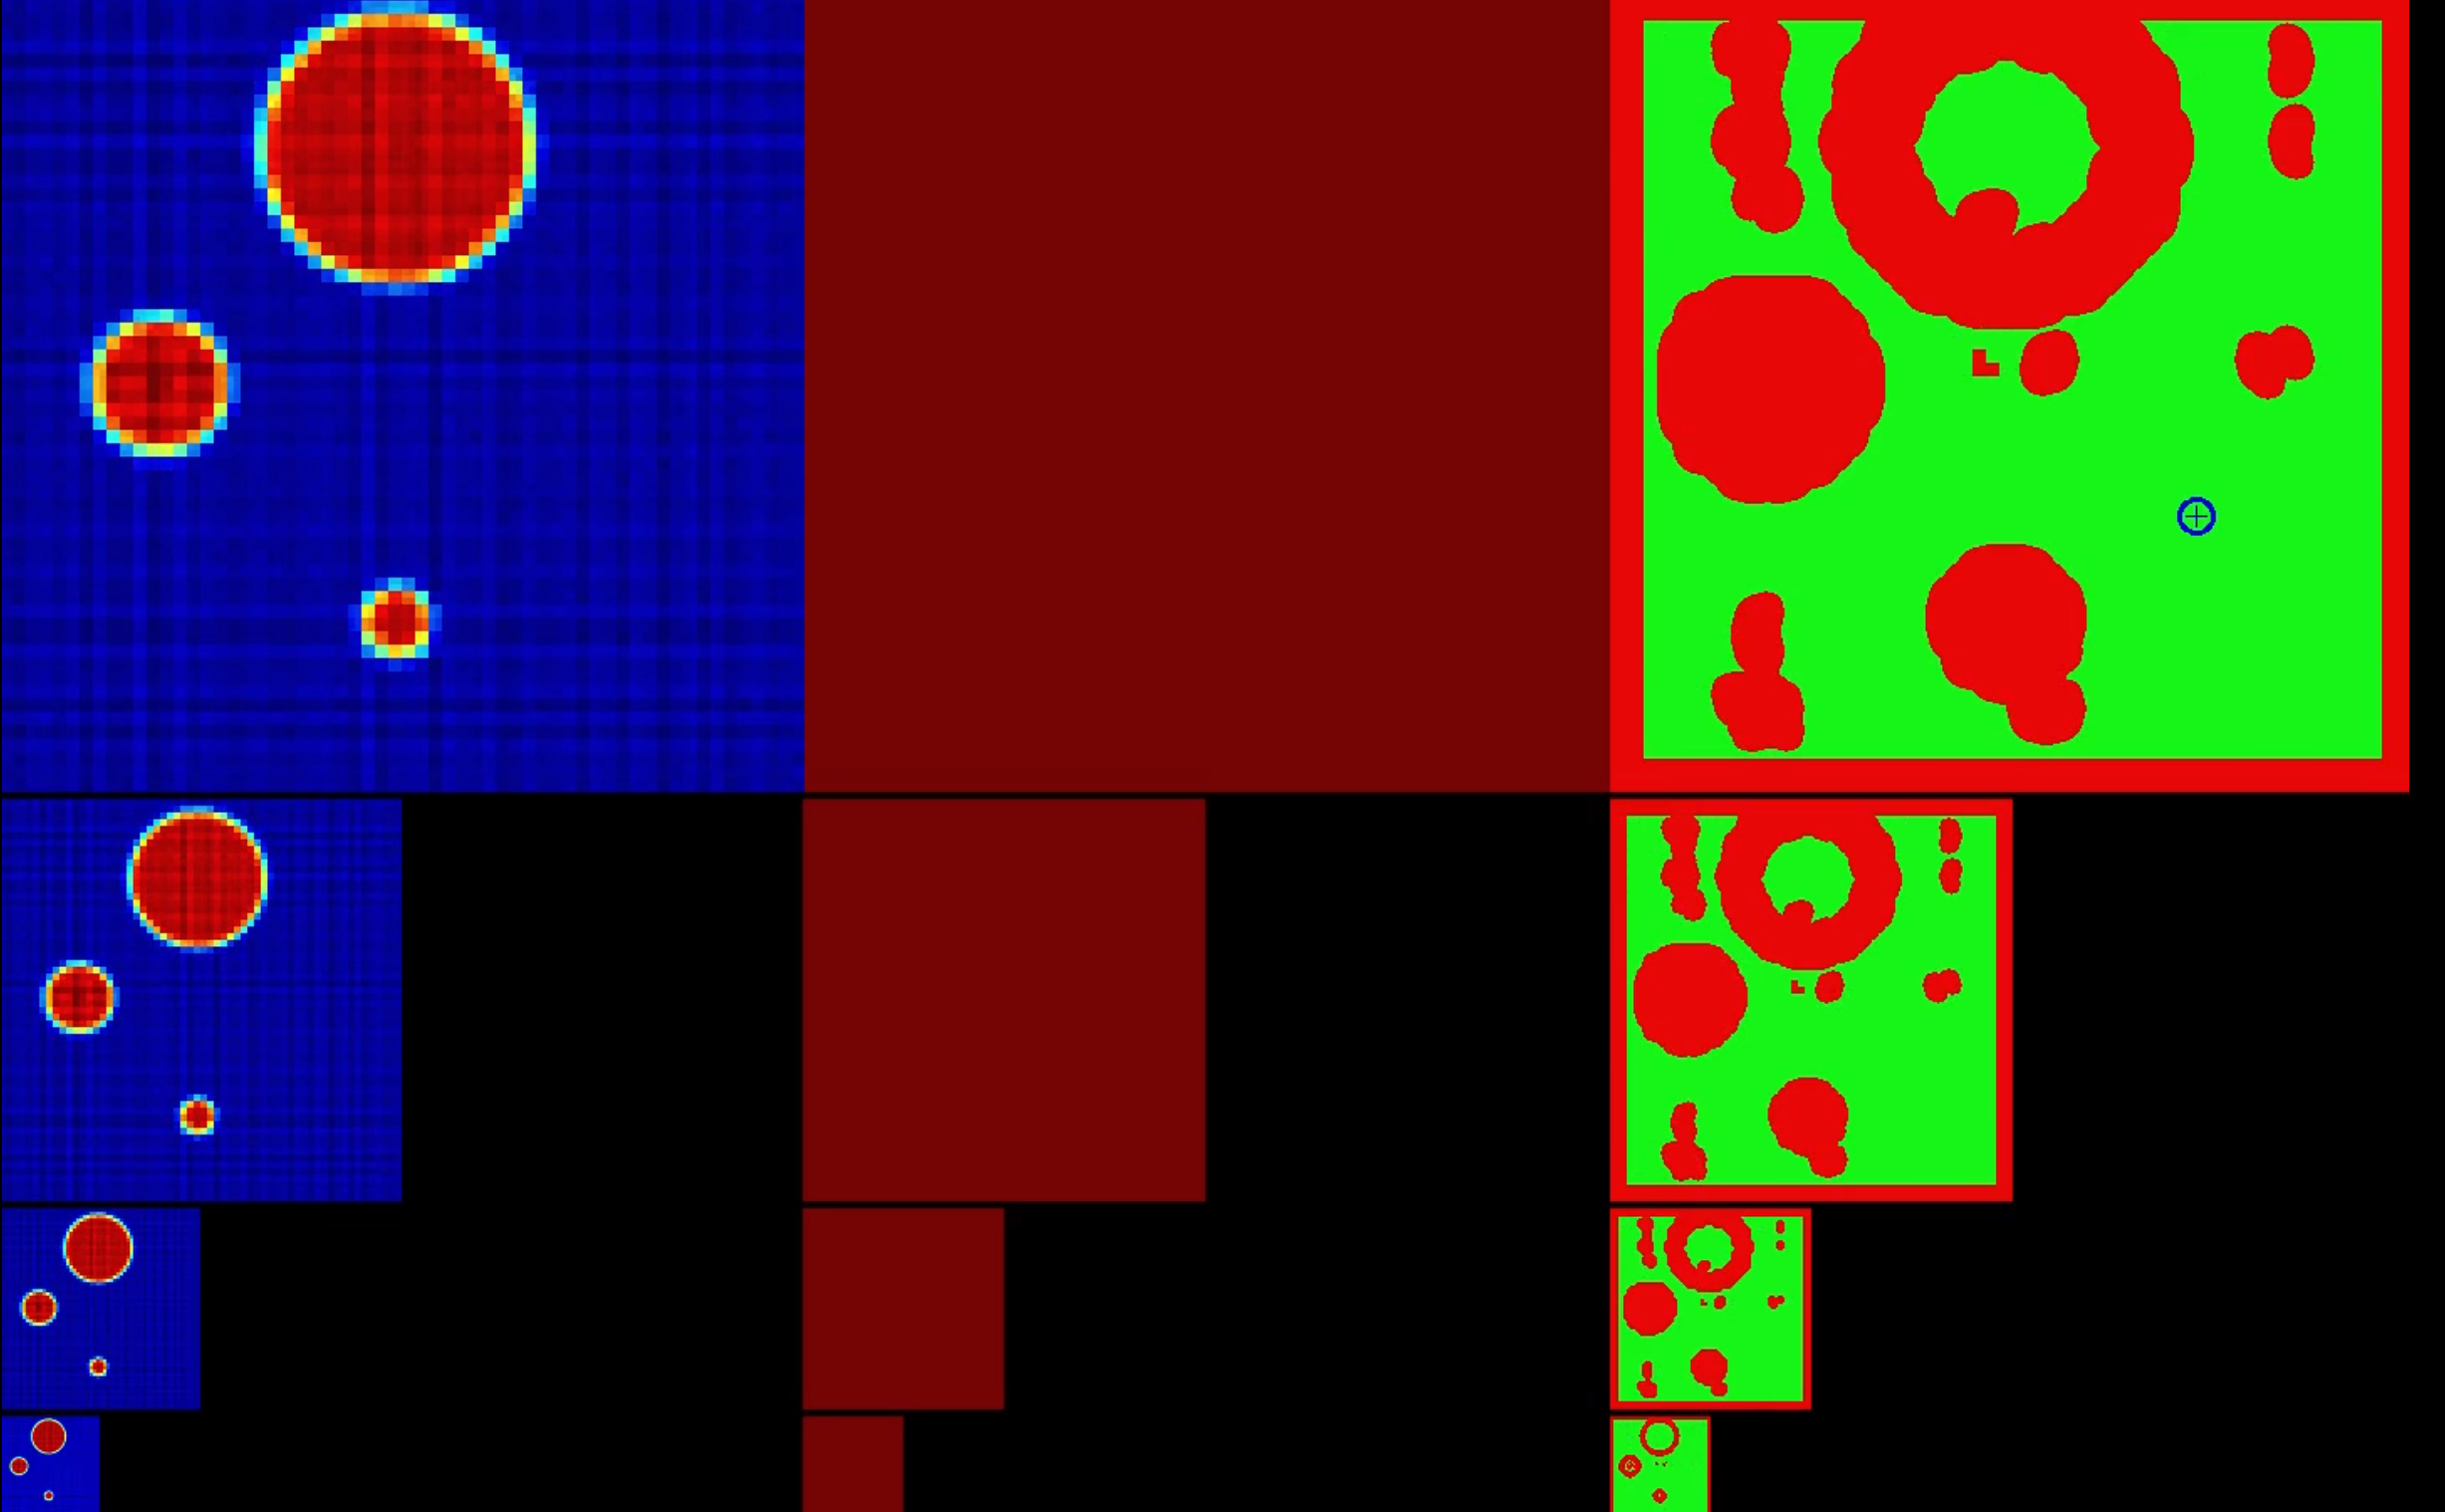
\includegraphics[scale=0.22]{images/methodology/SFM.png}
\caption{SFM result of the GT test}
\label{fig:gt_test_sfm}
\end{figure} 

Looking at \cref{fig:gt_test_gt} and \cref{fig:gt_test_sfm}, one can see, that, though the SFM quality is visibly worse, neither SFM nor GT detected the small rocks on the platforms. This can be seen because in both Debug images the center of the platforms was considered a landing site even though there was the rock which should definitely prevent the detection of a valid landing site.

Therefore, the ground truth depth could be used for the testing of the autonomous landing pipeline without making a landing site verification step at low altitudes redundant.

\clearpage %HERE
\section{Autonomous Landing Procedure}

Having implemented a stereo camera as a low altitude alternative to SFM, and after ensuring a correct ground truth comparison, the main contribution of this work could be tackled: Bringing the visual landing site pipeline together with the autonomy framework in order to achieve reliable autonomous landing in unknown terrain.

The manner of implementation for the autonomous landing sequence was more or less given by the system architectures which this work combines. The two crucial points of the methodology were the interface between the autonomy framework and the landing site detector and the implementation of the decision-making in the behavior tree of the landing node as well as the landing site manager.

\subsection{LSD - Autonomy Interface}

For the interface with the autonomy, both the autonomy and the landing site detection node had to be altered.

\begin{itemize}
    \item Landing site detection output

    Prior to this work, LSD only published one single landing site's location. To give the autonomy more information to make adequate decisions and to avoid the stagnation on a single overconfident landing site, LSD was changed to also first, publish three landing sites each iteration and secondly, yield additional characteristics with each output landing site.
    \item Landing site interface of the autonomy

    The autonomy framework was changed to correctly receive and handle the incoming landing sites with all the newly associated properties. The incoming candidates are ordered according to a novel landing site heuristic and further landing site handling concepts like re-detection and banishment were introduced.    
\end{itemize}

\subsection{Autonomous Landing Behavior}

As previously explained, the landing behavior in the autonomy framework is implemented using a behavior tree consisting of small modular and expandable actions. The existing BT framework and the available actions prior to this work are shown in \cref{subsec:setup:behavior_tree}.

The two paramount qualities in pursuit of which the landing behavior was designed are safety and efficiency. Naturally safety is the first most concern. We want a reliable autonomous landing procedure for the drone to repeatedly land safely. However, the more efficient it is, the more daring science missions can be designed and the faster the red planet can be explored in detail.

For the conceptual design of the autonomous landing behavior a fail-safe dogma was adopted meaning that the drone never moved both horizontally and vertically. Instead, any required traversal was preceded by an adequate ascent to a safe height and followed by a vertical descent to the desired altitude at the new location. Secondly the available landing site characteristics were used to enhance the overall efficiency. 




